\documentclass{standalone}
\usepackage{tikz}
\usetikzlibrary{patterns, positioning}


\begin{document}
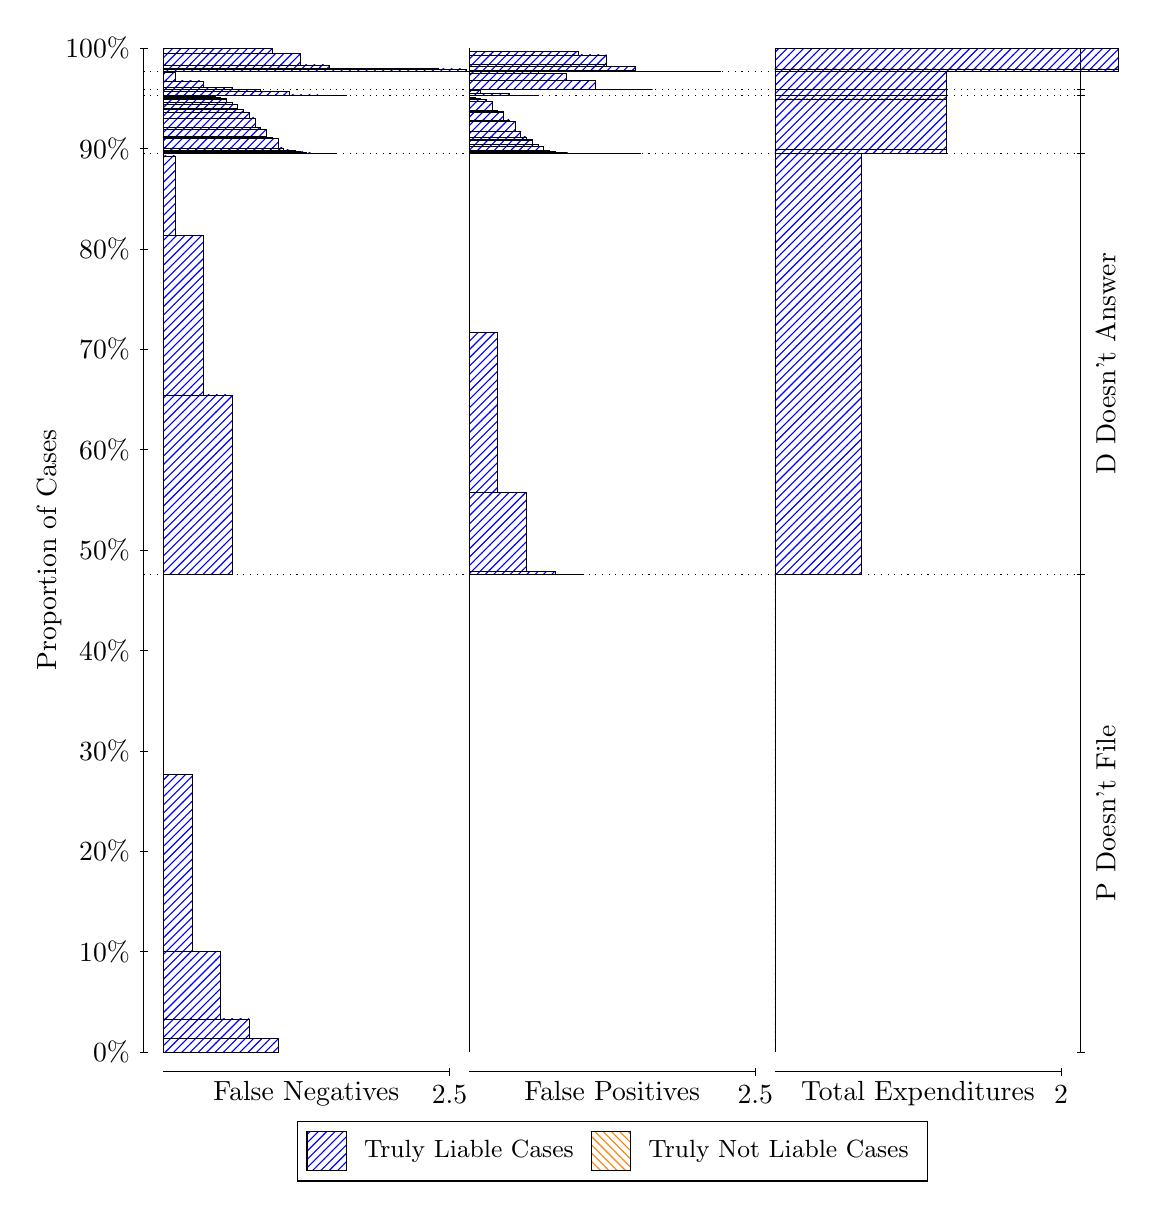
\begin{tikzpicture}
\draw[black, very thin] (1.5,1.75) -- (1.5,14.5);
\node[rotate=90, text=black, anchor=center] at (0.3, 8.125) {Proportion of Cases};
\draw[black, very thin] (1.45,1.75) -- (1.55,1.75);
\node[text=black, anchor=east] at (1.45, 1.75) {0\%};
\draw[black, very thin] (1.45,3.025) -- (1.55,3.025);
\node[text=black, anchor=east] at (1.45, 3.025) {10\%};
\draw[black, very thin] (1.45,4.3) -- (1.55,4.3);
\node[text=black, anchor=east] at (1.45, 4.3) {20\%};
\draw[black, very thin] (1.45,5.575) -- (1.55,5.575);
\node[text=black, anchor=east] at (1.45, 5.575) {30\%};
\draw[black, very thin] (1.45,6.85) -- (1.55,6.85);
\node[text=black, anchor=east] at (1.45, 6.85) {40\%};
\draw[black, very thin] (1.45,8.125) -- (1.55,8.125);
\node[text=black, anchor=east] at (1.45, 8.125) {50\%};
\draw[black, very thin] (1.45,9.4) -- (1.55,9.4);
\node[text=black, anchor=east] at (1.45, 9.4) {60\%};
\draw[black, very thin] (1.45,10.675) -- (1.55,10.675);
\node[text=black, anchor=east] at (1.45, 10.675) {70\%};
\draw[black, very thin] (1.45,11.95) -- (1.55,11.95);
\node[text=black, anchor=east] at (1.45, 11.95) {80\%};
\draw[black, very thin] (1.45,13.225) -- (1.55,13.225);
\node[text=black, anchor=east] at (1.45, 13.225) {90\%};
\draw[black, very thin] (1.45,14.5) -- (1.55,14.5);
\node[text=black, anchor=east] at (1.45, 14.5) {100\%};

\draw[black, very thin] (13.4,1.75) -- (13.4,14.5);
\draw[black, very thin] (13.35,1.75) -- (13.45,1.75);
\node[anchor=west] at (13.35, 1.75) {};
\draw[black, very thin] (13.35,7.8174) -- (13.45,7.8174);
\node[anchor=west] at (13.35, 7.8174) {};
\draw[black, very thin] (13.35,13.163) -- (13.45,13.163);
\node[anchor=west] at (13.35, 13.163) {};
\draw[black, very thin] (13.35,13.896) -- (13.45,13.896);
\node[anchor=west] at (13.35, 13.896) {};
\draw[black, very thin] (13.35,13.974) -- (13.45,13.974);
\node[anchor=west] at (13.35, 13.974) {};
\draw[black, very thin] (13.35,14.2) -- (13.45,14.2);
\node[anchor=west] at (13.35, 14.2) {};
\draw[black, very thin] (13.35,14.5) -- (13.45,14.5);
\node[anchor=west] at (13.35, 14.5) {};

\draw[black, very thin, pattern color=blue, pattern=north east lines] (1.75,1.75) rectangle (3.2033,1.9237);
\draw[black, very thin, pattern color=blue, pattern=north east lines] (1.75,1.9237) rectangle (2.84,2.1707);
\draw[black, very thin, pattern color=blue, pattern=north east lines] (1.75,2.1707) rectangle (2.4767,3.0274);
\draw[black, very thin, pattern color=blue, pattern=north east lines] (1.75,3.0274) rectangle (2.1133,5.2705);
\draw[black, very thin, pattern color=orange, pattern=north west lines] (1.75,5.2705) rectangle (1.75,5.2705);
\draw[black, very thin, pattern color=blue, pattern=north east lines] (1.75,5.2705) rectangle (1.75,7.8174);
\draw[black, very thin, pattern color=blue, pattern=north east lines] (1.75,7.8174) rectangle (2.622,10.096);
\draw[black, very thin, pattern color=blue, pattern=north east lines] (1.75,10.096) rectangle (2.2587,12.118);
\draw[black, very thin, pattern color=blue, pattern=north east lines] (1.75,12.118) rectangle (1.8953,13.13);
\draw[black, very thin, pattern color=orange, pattern=north west lines] (1.75,13.13) rectangle (1.75,13.13);
\draw[black, very thin, pattern color=blue, pattern=north east lines] (1.75,13.13) rectangle (1.75,13.163);
\draw[black, very thin, pattern color=blue, pattern=north east lines] (1.75,13.163) rectangle (3.93,13.164);
\draw[black, very thin, pattern color=blue, pattern=north east lines] (1.75,13.164) rectangle (3.7847,13.165);
\draw[black, very thin, pattern color=blue, pattern=north east lines] (1.75,13.165) rectangle (3.6393,13.167);
\draw[black, very thin, pattern color=blue, pattern=north east lines] (1.75,13.167) rectangle (3.5667,13.181);
\draw[black, very thin, pattern color=blue, pattern=north east lines] (1.75,13.181) rectangle (3.494,13.184);
\draw[black, very thin, pattern color=blue, pattern=north east lines] (1.75,13.184) rectangle (3.4213,13.198);
\draw[black, very thin, pattern color=blue, pattern=north east lines] (1.75,13.198) rectangle (3.3487,13.205);
\draw[black, very thin, pattern color=blue, pattern=north east lines] (1.75,13.205) rectangle (3.276,13.233);
\draw[black, very thin, pattern color=blue, pattern=north east lines] (1.75,13.233) rectangle (3.2033,13.348);
\draw[black, very thin, pattern color=blue, pattern=north east lines] (1.75,13.348) rectangle (3.1307,13.366);
\draw[black, very thin, pattern color=blue, pattern=north east lines] (1.75,13.366) rectangle (3.058,13.375);
\draw[black, very thin, pattern color=blue, pattern=north east lines] (1.75,13.375) rectangle (3.058,13.471);
\draw[black, very thin, pattern color=blue, pattern=north east lines] (1.75,13.471) rectangle (2.9853,13.494);
\draw[black, very thin, pattern color=blue, pattern=north east lines] (1.75,13.494) rectangle (2.9127,13.608);
\draw[black, very thin, pattern color=blue, pattern=north east lines] (1.75,13.608) rectangle (2.9127,13.613);
\draw[black, very thin, pattern color=blue, pattern=north east lines] (1.75,13.613) rectangle (2.84,13.688);
\draw[black, very thin, pattern color=blue, pattern=north east lines] (1.75,13.688) rectangle (2.7673,13.721);
\draw[black, very thin, pattern color=blue, pattern=north east lines] (1.75,13.721) rectangle (2.6947,13.734);
\draw[black, very thin, pattern color=blue, pattern=north east lines] (1.75,13.734) rectangle (2.6947,13.783);
\draw[black, very thin, pattern color=blue, pattern=north east lines] (1.75,13.783) rectangle (2.622,13.806);
\draw[black, very thin, pattern color=blue, pattern=north east lines] (1.75,13.806) rectangle (2.5493,13.854);
\draw[black, very thin, pattern color=blue, pattern=north east lines] (1.75,13.854) rectangle (2.5493,13.861);
\draw[black, very thin, pattern color=blue, pattern=north east lines] (1.75,13.861) rectangle (2.4767,13.874);
\draw[black, very thin, pattern color=blue, pattern=north east lines] (1.75,13.874) rectangle (2.404,13.875);
\draw[black, very thin, pattern color=blue, pattern=north east lines] (1.75,13.875) rectangle (2.404,13.883);
\draw[black, very thin, pattern color=blue, pattern=north east lines] (1.75,13.883) rectangle (2.3313,13.888);
\draw[black, very thin, pattern color=blue, pattern=north east lines] (1.75,13.888) rectangle (2.3313,13.889);
\draw[black, very thin, pattern color=blue, pattern=north east lines] (1.75,13.889) rectangle (2.2587,13.89);
\draw[black, very thin, pattern color=blue, pattern=north east lines] (1.75,13.89) rectangle (2.186,13.89);
\draw[black, very thin, pattern color=blue, pattern=north east lines] (1.75,13.89) rectangle (2.186,13.893);
\draw[black, very thin, pattern color=blue, pattern=north east lines] (1.75,13.893) rectangle (2.1133,13.894);
\draw[black, very thin, pattern color=blue, pattern=north east lines] (1.75,13.894) rectangle (2.0407,13.894);
\draw[black, very thin, pattern color=blue, pattern=north east lines] (1.75,13.894) rectangle (2.0407,13.896);
\draw[black, very thin, pattern color=blue, pattern=north east lines] (1.75,13.896) rectangle (1.968,13.896);
\draw[black, very thin, pattern color=blue, pattern=north east lines] (1.75,13.896) rectangle (1.8953,13.896);
\draw[black, very thin, pattern color=blue, pattern=north east lines] (1.75,13.896) rectangle (1.8227,13.896);
\draw[black, very thin, pattern color=orange, pattern=north west lines] (1.75,13.896) rectangle (1.75,13.896);
\draw[black, very thin, pattern color=blue, pattern=north east lines] (1.75,13.896) rectangle (1.75,13.896);
\draw[black, very thin, pattern color=blue, pattern=north east lines] (1.75,13.896) rectangle (4.0753,13.898);
\draw[black, very thin, pattern color=blue, pattern=north east lines] (1.75,13.898) rectangle (3.712,13.906);
\draw[black, very thin, pattern color=blue, pattern=north east lines] (1.75,13.906) rectangle (3.3487,13.948);
\draw[black, very thin, pattern color=blue, pattern=north east lines] (1.75,13.948) rectangle (2.9853,13.973);
\draw[black, very thin, pattern color=blue, pattern=north east lines] (1.75,13.973) rectangle (2.622,13.974);
\draw[black, very thin, pattern color=orange, pattern=north west lines] (1.75,13.974) rectangle (1.75,13.974);
\draw[black, very thin, pattern color=blue, pattern=north east lines] (1.75,13.974) rectangle (2.622,13.999);
\draw[black, very thin, pattern color=blue, pattern=north east lines] (1.75,13.999) rectangle (2.2587,14.082);
\draw[black, very thin, pattern color=blue, pattern=north east lines] (1.75,14.082) rectangle (1.8953,14.196);
\draw[black, very thin, pattern color=orange, pattern=north west lines] (1.75,14.196) rectangle (1.75,14.196);
\draw[black, very thin, pattern color=blue, pattern=north east lines] (1.75,14.196) rectangle (1.75,14.2);
\draw[black, very thin, pattern color=blue, pattern=north east lines] (1.75,14.2) rectangle (6.6913,14.2);
\draw[black, very thin, pattern color=blue, pattern=north east lines] (1.75,14.2) rectangle (6.328,14.2);
\draw[black, very thin, pattern color=blue, pattern=north east lines] (1.75,14.2) rectangle (5.9647,14.204);
\draw[black, very thin, pattern color=blue, pattern=north east lines] (1.75,14.204) rectangle (5.6013,14.235);
\draw[black, very thin, pattern color=blue, pattern=north east lines] (1.75,14.235) rectangle (5.238,14.245);
\draw[black, very thin, pattern color=blue, pattern=north east lines] (1.75,14.245) rectangle (4.8747,14.245);
\draw[black, very thin, pattern color=blue, pattern=north east lines] (1.75,14.245) rectangle (4.584,14.245);
\draw[black, very thin, pattern color=blue, pattern=north east lines] (1.75,14.245) rectangle (4.5113,14.245);
\draw[black, very thin, pattern color=blue, pattern=north east lines] (1.75,14.245) rectangle (4.2207,14.246);
\draw[black, very thin, pattern color=blue, pattern=north east lines] (1.75,14.246) rectangle (3.8573,14.287);
\draw[black, very thin, pattern color=blue, pattern=north east lines] (1.75,14.287) rectangle (3.494,14.432);
\draw[black, very thin, pattern color=blue, pattern=north east lines] (1.75,14.432) rectangle (3.1307,14.495);
\draw[black, very thin, pattern color=blue, pattern=north east lines] (1.75,14.495) rectangle (2.7673,14.5);
\draw[black, very thin, pattern color=blue, pattern=north east lines] (1.75,14.5) rectangle (2.404,14.5);
\draw[black, very thin, pattern color=blue, pattern=north east lines] (1.75,14.5) rectangle (2.0407,14.5);
\draw[black, very thin, pattern color=orange, pattern=north west lines] (1.75,14.5) rectangle (1.75,14.5);
\draw[black, very thin, pattern color=orange, pattern=north west lines] (5.6333,1.75) rectangle (5.6333,1.75);
\draw[black, very thin, pattern color=blue, pattern=north east lines] (5.6333,1.75) rectangle (5.6333,7.8174);
\draw[black, very thin, pattern color=orange, pattern=north west lines] (5.6333,7.8174) rectangle (7.0867,7.8174);
\draw[black, very thin, pattern color=blue, pattern=north east lines] (5.6333,7.8174) rectangle (7.0867,7.8174);
\draw[black, very thin, pattern color=blue, pattern=north east lines] (5.6333,7.8174) rectangle (6.7233,7.8499);
\draw[black, very thin, pattern color=blue, pattern=north east lines] (5.6333,7.8499) rectangle (6.36,8.8615);
\draw[black, very thin, pattern color=blue, pattern=north east lines] (5.6333,8.8615) rectangle (5.9967,10.884);
\draw[black, very thin, pattern color=blue, pattern=north east lines] (5.6333,10.884) rectangle (5.6333,13.163);
\draw[black, very thin, pattern color=orange, pattern=north west lines] (5.6333,13.163) rectangle (7.8133,13.163);
\draw[black, very thin, pattern color=blue, pattern=north east lines] (5.6333,13.163) rectangle (7.8133,13.163);
\draw[black, very thin, pattern color=orange, pattern=north west lines] (5.6333,13.163) rectangle (7.668,13.163);
\draw[black, very thin, pattern color=blue, pattern=north east lines] (5.6333,13.163) rectangle (7.668,13.163);
\draw[black, very thin, pattern color=orange, pattern=north west lines] (5.6333,13.163) rectangle (7.5227,13.163);
\draw[black, very thin, pattern color=blue, pattern=north east lines] (5.6333,13.163) rectangle (7.5227,13.163);
\draw[black, very thin, pattern color=blue, pattern=north east lines] (5.6333,13.163) rectangle (7.45,13.163);
\draw[black, very thin, pattern color=orange, pattern=north west lines] (5.6333,13.163) rectangle (7.3773,13.163);
\draw[black, very thin, pattern color=blue, pattern=north east lines] (5.6333,13.163) rectangle (7.3773,13.163);
\draw[black, very thin, pattern color=blue, pattern=north east lines] (5.6333,13.163) rectangle (7.3047,13.163);
\draw[black, very thin, pattern color=orange, pattern=north west lines] (5.6333,13.163) rectangle (7.232,13.163);
\draw[black, very thin, pattern color=blue, pattern=north east lines] (5.6333,13.163) rectangle (7.232,13.163);
\draw[black, very thin, pattern color=blue, pattern=north east lines] (5.6333,13.163) rectangle (7.1593,13.163);
\draw[black, very thin, pattern color=orange, pattern=north west lines] (5.6333,13.163) rectangle (7.0867,13.163);
\draw[black, very thin, pattern color=blue, pattern=north east lines] (5.6333,13.163) rectangle (7.0867,13.165);
\draw[black, very thin, pattern color=blue, pattern=north east lines] (5.6333,13.165) rectangle (7.014,13.166);
\draw[black, very thin, pattern color=orange, pattern=north west lines] (5.6333,13.166) rectangle (6.9413,13.166);
\draw[black, very thin, pattern color=blue, pattern=north east lines] (5.6333,13.166) rectangle (6.9413,13.169);
\draw[black, very thin, pattern color=blue, pattern=north east lines] (5.6333,13.169) rectangle (6.8687,13.17);
\draw[black, very thin, pattern color=orange, pattern=north west lines] (5.6333,13.17) rectangle (6.796,13.17);
\draw[black, very thin, pattern color=blue, pattern=north east lines] (5.6333,13.17) rectangle (6.796,13.171);
\draw[black, very thin, pattern color=blue, pattern=north east lines] (5.6333,13.171) rectangle (6.796,13.176);
\draw[black, very thin, pattern color=blue, pattern=north east lines] (5.6333,13.176) rectangle (6.7233,13.185);
\draw[black, very thin, pattern color=orange, pattern=north west lines] (5.6333,13.185) rectangle (6.6507,13.185);
\draw[black, very thin, pattern color=blue, pattern=north east lines] (5.6333,13.185) rectangle (6.6507,13.198);
\draw[black, very thin, pattern color=blue, pattern=north east lines] (5.6333,13.198) rectangle (6.578,13.253);
\draw[black, very thin, pattern color=blue, pattern=north east lines] (5.6333,13.253) rectangle (6.5053,13.276);
\draw[black, very thin, pattern color=blue, pattern=north east lines] (5.6333,13.276) rectangle (6.4327,13.325);
\draw[black, very thin, pattern color=blue, pattern=north east lines] (5.6333,13.325) rectangle (6.4327,13.338);
\draw[black, very thin, pattern color=blue, pattern=north east lines] (5.6333,13.338) rectangle (6.36,13.371);
\draw[black, very thin, pattern color=blue, pattern=north east lines] (5.6333,13.371) rectangle (6.2873,13.446);
\draw[black, very thin, pattern color=blue, pattern=north east lines] (5.6333,13.446) rectangle (6.2147,13.565);
\draw[black, very thin, pattern color=blue, pattern=north east lines] (5.6333,13.565) rectangle (6.142,13.588);
\draw[black, very thin, pattern color=blue, pattern=north east lines] (5.6333,13.588) rectangle (6.0693,13.684);
\draw[black, very thin, pattern color=blue, pattern=north east lines] (5.6333,13.684) rectangle (6.0693,13.693);
\draw[black, very thin, pattern color=blue, pattern=north east lines] (5.6333,13.693) rectangle (5.9967,13.711);
\draw[black, very thin, pattern color=blue, pattern=north east lines] (5.6333,13.711) rectangle (5.924,13.825);
\draw[black, very thin, pattern color=blue, pattern=north east lines] (5.6333,13.825) rectangle (5.8513,13.854);
\draw[black, very thin, pattern color=blue, pattern=north east lines] (5.6333,13.854) rectangle (5.7787,13.861);
\draw[black, very thin, pattern color=blue, pattern=north east lines] (5.6333,13.861) rectangle (5.706,13.875);
\draw[black, very thin, pattern color=blue, pattern=north east lines] (5.6333,13.875) rectangle (5.6333,13.896);
\draw[black, very thin, pattern color=orange, pattern=north west lines] (5.6333,13.896) rectangle (6.5053,13.896);
\draw[black, very thin, pattern color=blue, pattern=north east lines] (5.6333,13.896) rectangle (6.5053,13.897);
\draw[black, very thin, pattern color=blue, pattern=north east lines] (5.6333,13.897) rectangle (6.142,13.922);
\draw[black, very thin, pattern color=blue, pattern=north east lines] (5.6333,13.922) rectangle (5.7787,13.964);
\draw[black, very thin, pattern color=blue, pattern=north east lines] (5.6333,13.964) rectangle (5.6333,13.974);
\draw[black, very thin, pattern color=orange, pattern=north west lines] (5.6333,13.974) rectangle (7.9587,13.974);
\draw[black, very thin, pattern color=blue, pattern=north east lines] (5.6333,13.974) rectangle (7.9587,13.974);
\draw[black, very thin, pattern color=blue, pattern=north east lines] (5.6333,13.974) rectangle (7.5953,13.978);
\draw[black, very thin, pattern color=blue, pattern=north east lines] (5.6333,13.978) rectangle (7.232,14.092);
\draw[black, very thin, pattern color=blue, pattern=north east lines] (5.6333,14.092) rectangle (6.8687,14.174);
\draw[black, very thin, pattern color=blue, pattern=north east lines] (5.6333,14.174) rectangle (6.5053,14.2);
\draw[black, very thin, pattern color=orange, pattern=north west lines] (5.6333,14.2) rectangle (8.8307,14.2);
\draw[black, very thin, pattern color=blue, pattern=north east lines] (5.6333,14.2) rectangle (8.8307,14.2);
\draw[black, very thin, pattern color=blue, pattern=north east lines] (5.6333,14.2) rectangle (8.4673,14.2);
\draw[black, very thin, pattern color=orange, pattern=north west lines] (5.6333,14.2) rectangle (8.4673,14.2);
\draw[black, very thin, pattern color=blue, pattern=north east lines] (5.6333,14.2) rectangle (8.4673,14.2);
\draw[black, very thin, pattern color=blue, pattern=north east lines] (5.6333,14.2) rectangle (8.104,14.203);
\draw[black, very thin, pattern color=orange, pattern=north west lines] (5.6333,14.203) rectangle (8.104,14.203);
\draw[black, very thin, pattern color=blue, pattern=north east lines] (5.6333,14.203) rectangle (8.104,14.205);
\draw[black, very thin, pattern color=blue, pattern=north east lines] (5.6333,14.205) rectangle (7.7407,14.216);
\draw[black, very thin, pattern color=orange, pattern=north west lines] (5.6333,14.216) rectangle (7.7407,14.216);
\draw[black, very thin, pattern color=blue, pattern=north east lines] (5.6333,14.216) rectangle (7.7407,14.267);
\draw[black, very thin, pattern color=blue, pattern=north east lines] (5.6333,14.267) rectangle (7.3773,14.288);
\draw[black, very thin, pattern color=blue, pattern=north east lines] (5.6333,14.288) rectangle (7.3773,14.413);
\draw[black, very thin, pattern color=blue, pattern=north east lines] (5.6333,14.413) rectangle (7.014,14.453);
\draw[black, very thin, pattern color=blue, pattern=north east lines] (5.6333,14.453) rectangle (6.6507,14.454);
\draw[black, very thin, pattern color=orange, pattern=north west lines] (5.6333,14.454) rectangle (6.36,14.454);
\draw[black, very thin, pattern color=blue, pattern=north east lines] (5.6333,14.454) rectangle (6.36,14.454);
\draw[black, very thin, pattern color=blue, pattern=north east lines] (5.6333,14.454) rectangle (6.2873,14.454);
\draw[black, very thin, pattern color=orange, pattern=north west lines] (5.6333,14.454) rectangle (5.9967,14.454);
\draw[black, very thin, pattern color=blue, pattern=north east lines] (5.6333,14.454) rectangle (5.9967,14.455);
\draw[black, very thin, pattern color=orange, pattern=north west lines] (5.6333,14.455) rectangle (5.6333,14.455);
\draw[black, very thin, pattern color=blue, pattern=north east lines] (5.6333,14.455) rectangle (5.6333,14.5);
\draw[black, very thin, pattern color=orange, pattern=north west lines] (9.5167,1.75) rectangle (9.5167,1.75);
\draw[black, very thin, pattern color=blue, pattern=north east lines] (9.5167,1.75) rectangle (9.5167,7.8174);
\draw[black, very thin, pattern color=orange, pattern=north west lines] (9.5167,7.8174) rectangle (10.607,7.8174);
\draw[black, very thin, pattern color=blue, pattern=north east lines] (9.5167,7.8174) rectangle (10.607,13.163);
\draw[black, very thin, pattern color=orange, pattern=north west lines] (9.5167,13.163) rectangle (11.697,13.163);
\draw[black, very thin, pattern color=blue, pattern=north east lines] (9.5167,13.163) rectangle (11.697,13.216);
\draw[black, very thin, pattern color=orange, pattern=north west lines] (9.5167,13.216) rectangle (11.697,13.216);
\draw[black, very thin, pattern color=blue, pattern=north east lines] (9.5167,13.216) rectangle (11.697,13.853);
\draw[black, very thin, pattern color=orange, pattern=north west lines] (9.5167,13.853) rectangle (11.697,13.853);
\draw[black, very thin, pattern color=blue, pattern=north east lines] (9.5167,13.853) rectangle (11.697,13.896);
\draw[black, very thin, pattern color=orange, pattern=north west lines] (9.5167,13.896) rectangle (11.697,13.896);
\draw[black, very thin, pattern color=blue, pattern=north east lines] (9.5167,13.896) rectangle (11.697,13.974);
\draw[black, very thin, pattern color=orange, pattern=north west lines] (9.5167,13.974) rectangle (11.697,13.974);
\draw[black, very thin, pattern color=blue, pattern=north east lines] (9.5167,13.974) rectangle (11.697,14.2);
\draw[black, very thin, pattern color=orange, pattern=north west lines] (9.5167,14.2) rectangle (13.877,14.2);
\draw[black, very thin, pattern color=blue, pattern=north east lines] (9.5167,14.2) rectangle (13.877,14.235);
\draw[black, very thin, pattern color=orange, pattern=north west lines] (9.5167,14.235) rectangle (13.877,14.235);
\draw[black, very thin, pattern color=blue, pattern=north east lines] (9.5167,14.235) rectangle (13.877,14.5);
\draw[black, dotted] (1.5,7.8174) -- (13.4,7.8174);
\draw[black, dotted] (1.5,13.163) -- (13.4,13.163);
\draw[black, dotted] (1.5,13.896) -- (13.4,13.896);
\draw[black, dotted] (1.5,13.974) -- (13.4,13.974);
\draw[black, dotted] (1.5,14.2) -- (13.4,14.2);
\draw[black, very thin] (1.75,1.5) -- (5.3833,1.5);
\node[text=black, anchor=north] at (3.5667, 1.5) {False Negatives};
\draw[black, very thin] (5.3833,1.45) -- (5.3833,1.55);
\node[text=black, anchor=north] at (5.3833, 1.45) {2.5};

\draw[black, very thin] (5.6333,1.5) -- (9.2667,1.5);
\node[text=black, anchor=north] at (7.45, 1.5) {False Positives};
\draw[black, very thin] (9.2667,1.45) -- (9.2667,1.55);
\node[text=black, anchor=north] at (9.2667, 1.45) {2.5};

\draw[black, very thin] (9.5167,1.5) -- (13.15,1.5);
\node[text=black, anchor=north] at (11.333, 1.5) {Total Expenditures};
\draw[black, very thin] (13.15,1.45) -- (13.15,1.55);
\node[text=black, anchor=north] at (13.15, 1.45) {2};

\node[text=black, centered, rotate=90] at (13.72, 4.7837) {P Doesn't File};
\node[text=black, centered, rotate=90] at (13.72, 10.49) {D Doesn't Answer};





\draw (7.449999999999999,1.5) node[draw=none] (baseCoordinate) {};
\begin{scope}[align=center]
        \matrix[scale=0.5, draw=black, below=0.5cm of baseCoordinate, nodes={draw}, column sep=0.1cm]{
            \node[rectangle, draw, minimum width=0.5cm, minimum height=0.5cm, pattern color=blue, pattern=north east lines] {}; &
            \node[draw=none, font=\small, text=black] (B) {Truly Liable Cases}; &
            \node[rectangle, draw, minimum width=0.5cm, minimum height=0.5cm, pattern color=orange, pattern=north west lines] {}; &
            \node[draw=none, font=\small, text=black] (B) {Truly Not Liable Cases}; \\
            };
\end{scope}

\end{tikzpicture}
\end{document}